\subsection{参数自洽、失效边界与终点收队}
\subsubsection{目标源适配契约与输入冲突}
方式二可用marker或pose目标源，但同一\texttt{target\_\allowbreak pose}不能同时由两个互不协调的适配器发布。marker来自TonyPi背部ALVAR实际观测，pose来自前车地图定位；二者目标身份、误差结构与可见条件不同。切换来源必须在实验元数据中登记，不把两种来源得到的结果混为一次独立方法。
\begin{table}[H]\centering\small\begin{tabularx}{\linewidth}{p{28mm}YY}\toprule 目标源 & 输入前提 & 主要误差/失效\\\midrule
marker & ID正确、尺寸标定、测量时间TF & 遮挡、角点误差、内参/外参错误\\
pose & 前车地图原点一致、定位有效 & 协方差异常、跳变、时间过期\\
公共输出 & frame=map、严格递增stamp & 坐标错用、旧观测刷新、双源竞争\\\bottomrule\end{tabularx}\caption{目标适配器的共同契约和差异。}\end{table}
\texttt{map\_\allowbreak follower}接受的是map中的目标点，不会从TonyPi动作次数估算位置。输入缺失时取消目标，历史缓存不是无期限继续运动的许可。上层身份有效与下层几何可行均成立，才具有继续推进的必要条件。
\source{\code{marker_target.py}；\code{pose_relay.py}；\code{follow_map.launch}。}

\subsubsection{定位质量门限的统计量纲}
\texttt{localization\_\allowbreak ok}检查36元协方差数组中x、y、yaw的对角值，要求有限、非负并小于阈值。0.25的平移协方差上限量纲是平方米，不是0.25米位置误差；0.35的角协方差是弧度平方。对角值通过只说明AMCL自己报告分布未过宽，不能保证全局匹配正确。
\begin{equation}
\sigma_x=\sqrt{\Sigma_{xx}},\qquad \Sigma_{xx},\Sigma_{yy}\le0.25\ \mathrm m^2,\quad\Sigma_{\psi\psi}\le0.35\ \mathrm{rad}^2.
\end{equation}
其中标准差与协方差的关系应理解为定义上的平方根，不把它当外部真实误差界。重复长走廊可能让错误初值表现得很自信，因而还要观察scan-map重合、外部地标和实际运动。静止定位请求只用新扫描更新，不能给没有扫描的前车制造新鲜定位。实验记录要区分内部质量指标和独立真值误差。
\source{\code{planning.py}：localization\_ok；\code{localization_refresh.py}。}

\subsubsection{路径缓存的时间复杂度与采样取舍}
Trail添加每个新点时计算现有折线总长度，必要时从前端删除旧点，behind再反向遍历选点。对N个缓存点，一次长度扫描和选点都是线性量级；\texttt{max\_\allowbreak length}与spacing使长期存储有界。默认20 m和0.08 m对应的理想规模约数百点，但转角密度和噪声会影响实际点数。
\begin{equation}
N\ \text{量级约为}\ L_{\max}/s_{\min},\qquad C_{\mathrm{add}},C_{\mathrm{behind}}=O(N).
\end{equation}
采样间距太小会增加抖动与存储，太大则用长边跨过真实弯曲轨迹。跳变阈值应与目标最大速度和观测间隔相容；相同0.8 m阈值对高频和低频数据意味着不同允许运动。若未来更新频率提高，可维护累计弧长以降低重复计算，但当前代码没有实现该优化，报告只作为可检验改进方向提出。
\source{\code{competition_core/planning.py}：Trail.add、Trail.behind。}

\subsubsection{轨迹采样间距与转角几何}
图\ref{fig:trail-sampling}向实际\code{Trail.add}函数输入同一条人工定义的折线路径，仅改变最小采样间距。这样可以把“轨迹缓存如何表示转角”与实际定位噪声分开，观察函数本身的保留点行为。背景灰线为给定路径，青色点线为函数保留的轨迹。
\begin{figure}[H]\centering
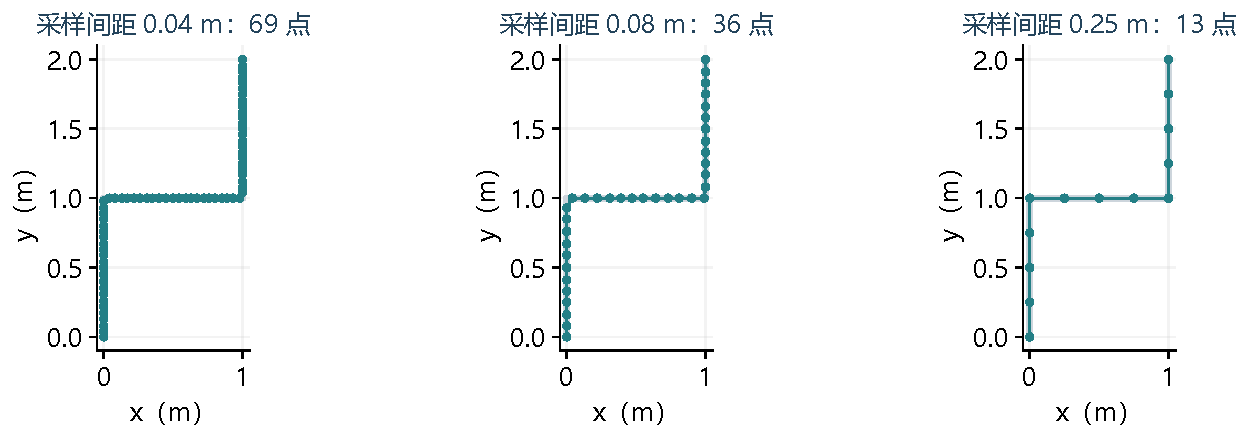
\includegraphics[width=.97\linewidth,height=.25\textheight,keepaspectratio]{figures/enriched/trail_sampling.pdf}
\caption{实际轨迹缓存函数对不同采样间距的响应；输入为明确给定的合成折线，不是实测轨迹。}\label{fig:trail-sampling}
\end{figure}
较大间距减少保留点数量，也可能使转角附近由一条较长线段连接，从而偏离原始折线。较小间距增加空间分辨率，但不能抑制定位噪声；当噪声本身达到间距量级时，路径弧长还可能被抖动放大。因此0.08\,m应视为需要结合定位质量和弯道尺度标定的配置，而不是任意场地都最优的常数。
\source{\code{planning.py}：Trail.add；图源\code{enrich_report_figures.py}。}

\subsubsection{DWA代价权衡和局部失败解释}
当前局部规划在非全向差速限制下采样线速度和角速度，没有横向运动。\texttt{path\_\allowbreak distance\_\allowbreak bias}、\texttt{goal\_\allowbreak distance\_\allowbreak bias}和\texttt{occdist\_\allowbreak scale}分别影响靠近全局路、追目标和避障。改变权重会改变通道内贴墙、犹豫或切角倾向，但这些是需要实验验证的行为假设，不是调某个权重必然改善的结论。
\begin{table}[H]\centering\small\begin{tabularx}{\linewidth}{p{33mm}YY}\toprule 可调因素 & 预期影响 & 应记录的代价\\\midrule
速度/预测时长 & 反应范围与前视距离 & 停止余量、计算、目标出视野\\
路径/目标权重 & 保持路线与追近目标 & 横向误差、切角、抢占次数\\
障碍权重/膨胀 & 增加围挡余量 & 窄道不可行、等待时间\\
目标刷新间隔 & 降低反复重规划 & 响应迟滞、终点小位移遗漏\\\bottomrule\end{tabularx}\caption{导航调参应采用的权衡记录。}\end{table}
失败应结合actionlib状态与地图诊断。ABORTED可能是路径/控制超时，不必然说明感知没看见；REJECTED可能是目标不可用；LOST是客户端失去状态。当前程序将其锁定停车，不能用后台旋转恢复掩盖目标丢失。改进应保留失败样本，比较同场地独立重复，而非仅展示成功的一次。
\source{\code{move_base.yaml}；\code{map_follower.py}导航状态分支。}

\subsubsection{终点收队与目标末端冻结}
TonyPi放下物块不代表TurtleBot已进入终点。地图follower在mission=done且距后置点小于\texttt{finish\_\allowbreak tolerance}时置finished，再取消导航。它未检查整车足迹在终点多边形中，也没有强制连续停稳保持时间；因此需要外部终点区域判定与实测速度证据。

目标限频还有末端问题：最新后置点移动小于\texttt{goal\_\allowbreak shift}时可能不发送新目标，机器人停在旧点附近，而完成判断仍对最新点计算。是否实际导致等待取决于阈值、容差和场景，应通过终点小位移用例验证，不能直接宣称必然失败。当前报告引用RGB-D的\texttt{need\_\allowbreak goal}图仅作算法比较，明确它不是地图follower已具备的最终目标修正。
\begin{equation}
G_{\mathrm{mapfinish}}=(\mathrm{mission}=\mathrm{done})\land\|p_r-g_{\mathrm{trail}}\|\le\epsilon_f.
\end{equation}
正式全队完成还要联合四车实际到达与停稳，保留Pi状态直到末车完成。终点区域需同时容纳队列的外包络与间隔，这一场地约束不能只按机器人中心点判断。
\source{\code{map_follower.py}：finished、goal\_shift与finish\_tolerance。}

\subsubsection{终点刷新与完成容差的边界示例}
图\ref{fig:terminal-threshold}给出一个一维几何示例：机器人已到旧目标，最新回退目标前移0.24\,m。位移小于0.25\,m重发门限，却大于0.20\,m完成容差；若其他条件没有触发新目标，就可能出现“没有刷新目标，也未满足完成”的等待。该示例用于解释两个阈值的关系，不表明本次视频已经发生此现象。
\begin{figure}[H]\centering
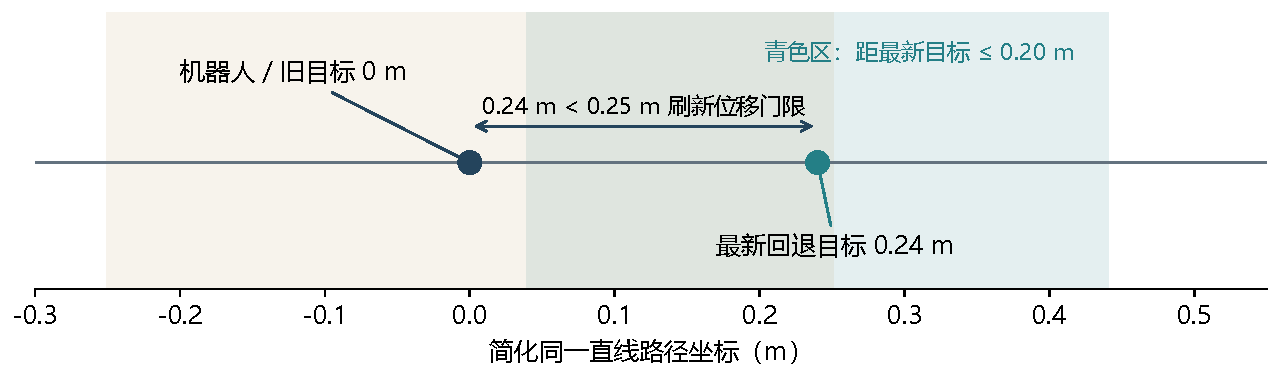
\includegraphics[width=.95\linewidth,height=.23\textheight,keepaspectratio]{figures/enriched/terminal_threshold.pdf}
\caption{终点目标刷新位移与完成容差的简化边界示例。机器人和旧目标重合，青色区为最新目标的完成邻域。}\label{fig:terminal-threshold}
\end{figure}
边界问题取决于最新目标、旧目标与实际机器人位置三者的关系，而不是只比较两个配置数值。验证时应保留最后一次发送的导航目标和当前回退点，在进入\code{done}前后分别检查刷新条件与完成条件。可能的改进包括终点阶段降低位移门限或强制发送最终目标，但这些需要单独实现和验证，本文不将建议写成现有功能。
\source{\code{map_follower.py}：goal\_shift与finish\_tolerance。}

\subsubsection{从故障命令到物理停稳的时间分解}
软件保护有多个时刻：故障发生、上游发现、许可撤销、门控发布零速、底盘实际停稳。日志若只记录零Twist发布时间，会低估真实停止延迟；电机控制、电池、地面摩擦和惯性影响最后一段。门控的0.4/0.5 s时限只是部分检测预算，不等于最大物理停机时间。
\begin{equation}
T_{\mathrm{stop}}=T_{\mathrm{detect}}+T_{\mathrm{transport}}+T_{\mathrm{gate}}+T_{\mathrm{brake}},\qquad d_s\approx vT_{\mathrm{delay}}+\frac{v^2}{2a_b}.
\end{equation}
距离表达是假定匀减速的分析模型，a应由实测保守下界而不是DWA加速度配置替代。方式二当前基于扫描阈值门控，不实现RGB-D方案的全方向停止包络。现场建议先低速直道测试断目标、断许可、断扫描，记录独立里程计/外部视频停稳，再进入围挡转角。
\source{\code{velocity_gate.py}；底盘实测制动记录。}
